\documentclass{article}
\usepackage[utf8]{inputenc}

\title{Rendering Sample Document}
\author{mattj23}
\date{October, 2019}

\usepackage{natbib}
\usepackage{graphicx}

\begin{document}

\maketitle

\section{Overview}
This is a sample document, renderable to a pdf by a latex compiler. Inside this docment is a lot of words, and these words are combined together to make paragraphs, and the paragraphs together make sections. Each section manages to use a great deal of words without communicating anything in particular.

By combining lots of words without meaning, we produce the illusion of meaningful content. Meaningless atomic units of information combine in such a way that they appear to transcend their meaningless, and meaning looks as if it is materialized from the heart of meaninglessness itself and made concrete in the assemblage of now suddenly structured content.  But in so doing, meaning is made to be the condition of segregation of meaning from its negation, as merely an abstract, or an ideal ideality.  And this change from meaning to the negation of meaning and its reversal in the negation of anti-meaning into meaning is simply the appearance of meaning as it originates conceptually from the dialectic.  In such the real identify of meaning and its cohesion with the ideality is made to be its ideal of specific specificness.

But do not be deceived, there is no actual content here. Nothing is produced on these pages, nor is anything communicated. Reading these sentences are as wasteful of time as writing them was.

\section{Why would you do this?}
As it would happen, there needed to be some payload of example files to be used in the testing of this project, and lorum ipsum ends up being quite boring.  If you've read this far you have indeed wasted your time and, in accordance with the warning in the previous section, you have nobody to blame except yourself.


\begin{figure}[h!]
\centering
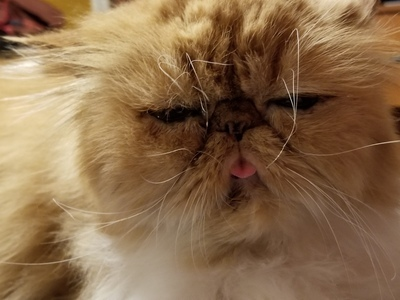
\includegraphics[scale=1.7]{cat}
\caption{This is a consolatory image of my cat.}
\label{fig:cat}
\end{figure}

\end{document}
